\documentclass[11pt]{article}
\usepackage[margin=0.9in]{geometry}
\usepackage{amsmath, amssymb}
\usepackage{graphicx}
\usepackage{float}
\usepackage{booktabs}
\usepackage[font=small,labelfont=bf]{caption}
\usepackage{xcolor}
\usepackage{enumitem}
\usepackage{multirow}
\usepackage[colorlinks=true,linkcolor=blue!55!black,citecolor=blue!55!black,urlcolor=blue!55!black]{hyperref}
\setlist[itemize]{leftmargin=1.4em, itemsep=0.12em, topsep=0.2em}

% Lightweight, mode-safe unit macros (avoid siunitx dependency)
\newcommand{\SI}[2]{#1\,\text{#2}}
\newcommand{\si}[1]{\text{#1}}
\newcommand{\SIrange}[3]{#1--#2\,\text{#3}}
\newcommand{\fmax}{\ensuremath{F_{\mathrm{max}}}}
\newcommand{\nneg}{\ensuremath{n_{\mathrm{neg}}}}
\newcommand{\evA}{\ensuremath{\,\text{eV/\AA}}}
\renewcommand{\pm}{\ensuremath{\,\text{pm}}}

\title{\Large\textbf{Simplicity as a Feature: Robust Transition-State Search\\[2pt]
by Gentlest Ascent Dynamics with Cheap Analytic Hessians}}
\author{}
\date{\today}

\begin{document}
\maketitle
\thispagestyle{empty}
\vspace{-2.2em}

% =====================================================================
\section*{Abstract}
% =====================================================================
\noindent
Machine-learned interatomic potentials (MLIPs) make analytic Hessians cheap
($\approx\!\SI{0.06}{s}$/structure with HIP \cite{hip}), so the bottleneck in
transition-state (TS) search is no longer the Hessian but the \emph{step}. We
use the minimal choice --- first-order Gentlest Ascent Dynamics (GAD) on the
lowest eigenvector of the Eckart-projected analytic Hessian, a Cartesian step
with no trust region, quasi-Newton update, RFO, or eigenvector prediction. Our
primary metric is the \emph{IRC convergence rate} (forward and
backward IRC must graph-match the intended reactant and product), on 287
Transition1x test reactions from perturbed-saddle guesses (10--\SI{200}{pm}).

\vspace{0.3em}
\noindent\textbf{Highlights}
\begin{itemize}
\item \textbf{Crossover, not a point.} GAD is statistically indistinguishable
  from the strongest Sella baseline when the guess is good (McNemar $p\!\approx\!1.0$,
  $\le\!\SI{50}{pm}$) and pulls significantly ahead as it degrades
  ($p\!<\!10^{-4}$ by 150--\SI{200}{pm}; \textbf{+21.6~pp intended at \SI{200}{pm}},
  45.3\% vs.\ 23.7\%). The same crossover holds for \fmax/\nneg convergence and across
  \fmax{} thresholds.
\item \textbf{Mechanism (corrected).} \emph{No} method converges to an
  unintended (wrong-basin) saddle --- unintended $\approx 0/287$ for all three.
  GAD's edge is recovering the full two-sided reaction more often; Sella's
  high-noise loss is non-convergence + one-sided (partial) saddles, not wrong
  basins.
\item \textbf{Honest cost.} First-order GAD cannot tighten \fmax{} below
  $\approx\!0.01\evA$; no step budget removes it. This plateau lives on the
  \emph{secondary} (convergence) axis only.
\item \textbf{Hybrid.} A GAD$\rightarrow$Newton switch removes the plateau, wins
  wall-time per converged TS ($1.4$--$3\times$) and geometry (tightest p95
  RMSD), and inherits GAD's chemistry.
\item \textbf{Scope boundary.} Robustness is demonstrated for \emph{perturbed-saddle}
  guesses. From a reactant start the GAD family is weak (hybrid $\sim$2\%) and
  Sella wins --- GAD needs to start near the saddle for the reaction mode to be
  identifiable.
\end{itemize}

% =====================================================================
\section{Introduction}

\begin{itemize}
\item TSs are index-1 saddle points; locating them needs curvature (the Hessian,
  or at least its leftmost eigenpair). \emph{Ab initio} Hessians are expensive,
  so optimizers avoid them: dimer \cite{dimer}, eigenvector-following / P-RFO
  \cite{cerjanmiller,banerjee,baker}, Sella's iterative partial-Hessian
  diagonalization \cite{sella2019,sella2022}, and recent ML prediction of the
  Hessian \cite{newtonnet,hip} or its leftmost eigenvector \cite{lmhe}.
\item \textbf{The premise has changed.} With MLIPs the analytic Hessian is cheap
  ($\approx\!\SI{0.06}{s}$ for HIP \cite{hip}). The bottleneck becomes the
  \textbf{step}. Trust-region/Newton jumps ($\mathcal{O}(0.1\,$\AA$)$) are
  optimal near a quadratic saddle but fragile from a poor guess.
\item \textbf{This work.} Given a cheap exact Hessian, discard P-RFO, trust
  radii, QN, and eigenvector prediction; step with first-order GAD \cite{gad}.
  Score success by IRC-validated \emph{intended} recovery \cite{newtonnet,lmhe},
  not mere convergence. Thesis: \emph{in the MLIP regime you need not avoid the
  Hessian --- you need to step more carefully with it.}
\end{itemize}

% =====================================================================
\section{Methods}\label{sec:methods}
% =====================================================================
\textbf{GAD dynamics.} With forces $\mathbf{F}=-\nabla E$ and $\mathbf{v}_1$ the
lowest eigenvector of the mass-weighted, Eckart-projected Hessian,
\begin{equation}
\dot{\mathbf{x}} = \bigl(\mathbf{I} - 2\,\mathbf{v}_1\mathbf{v}_1^{\!\top}\bigr)\mathbf{F}
= \mathbf{F} - 2(\mathbf{F}\!\cdot\!\mathbf{v}_1)\,\mathbf{v}_1 ,
\qquad
\mathbf{x}_{k+1} = \mathbf{x}_k + dt\,\dot{\mathbf{x}} .
\label{eq:gad}
\end{equation}
\begin{itemize}
\item \textbf{Step:} fixed-$dt$ explicit Euler ($dt\!\in\!\{0.003,0.005,0.007\}$;
  representative 0.005), Cartesian, no history/trust-region/line-search; mode
  tracked by max overlap; per-atom cap \SI{0.35}{\AA}.
\item \textbf{Potential:} HIP \cite{hip}, an $SE(3)$-equivariant MLIP returning
  the analytic Hessian ($\approx\!\SI{0.06}{s}$); not trained on Transition1x
  (held out); Hessian recomputed every step.
\item \textbf{Eckart projection:} remove the 6 translation/rotation modes in
  mass-weighted coordinates, diagonalize the reduced $(3N\!-\!6)$ Hessian; single
  most important robustness ingredient. (Cartesian vs.\ MW step: $\le 0.35$~pp.)
\item \textbf{Hybrid GAD--Newton:} walk with Eq.~\eqref{eq:gad}; near a clean
  index-1 saddle ($\nneg{=}1$, small force) switch to a trust-radius-capped
  eigenvector-following Newton step on the same analytic Hessian.
\item \textbf{Benchmark:} 287 Transition1x \cite{transition1x} test reactions;
  start = true saddle + isotropic Gaussian noise
  $\sigma\!\in\!\{10,30,50,100,150,200\}\pm$; baseline = Sella \cite{sella2022}
  (strongest config: Cartesian + Eckart, exact Hessian/step;
  Appendix~\ref{app:sella}).
\end{itemize}

\noindent\textbf{Two metrics, kept deliberately separate.}
\begin{itemize}
\item \textbf{IRC convergence rate --- primary.} Did we find the
  \emph{right} TS? After optimization, follow Sella's IRC \cite{sella2022}
  forward/backward and graph-match each endpoint (Open~Babel connectivity + VF2)
  to the labelled reactant/product. Outcomes (after \cite{newtonnet,lmhe}):
  \emph{intended} (both endpoints match), \emph{partially intended} (one),
  \emph{unintended} (valid saddle, other reaction), \emph{no reaction}
  (collapsed to a minimum), \emph{TS error} (no convergence). This is the
  chemically meaningful score and our headline metric.
\item \textbf{\fmax/\nneg convergence rate --- secondary.} Did the optimizer reach
  \emph{a} first-order saddle at all: $\nneg{=}1 \wedge \fmax{<}\tau$ (default
  $\tau=0.01\evA$; threshold family in Appendix~\ref{app:crit}). A pure-geometry
  check, necessary but \emph{insufficient} for the intended reaction; reported
  separately in Section~\ref{sec:fmax}, not alongside the primary metric.
\end{itemize}

% =====================================================================
\section{Results}
% =====================================================================
\subsection{Primary result: IRC convergence (IRC) crosses over with guess quality}\label{sec:primary}

\begin{figure}[H]\centering
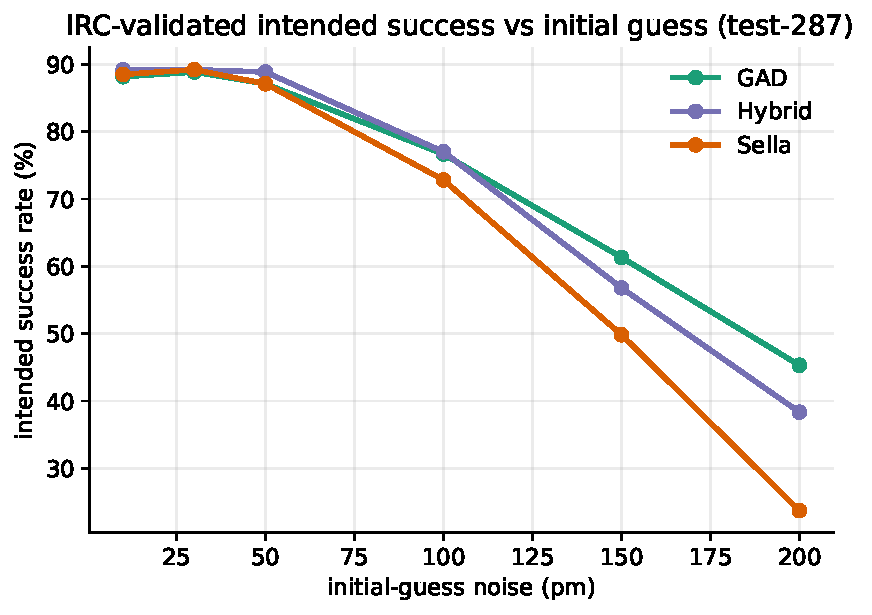
\includegraphics[width=0.72\textwidth]{figures_new/fig_intended_success_single.pdf}
\caption{\textbf{Primary metric: IRC convergence rate vs.\
initial-guess noise}, $n=287$. \emph{$x$-axis:} isotropic Gaussian perturbation
of the true saddle (10--\SI{200}{pm}). \emph{$y$-axis:} \% of the 287 reactions
whose forward and backward IRC graph-match \emph{both} the intended reactant and
product. One line each for GAD, the hybrid, and the strongest Sella baseline. The
three methods coincide while the guess is good; GAD and the hybrid retain far
more intended reactions as it degrades. (\fmax/\nneg convergence is shown separately
in Fig.~\ref{fig:conv}.)}
\label{fig:primary}
\end{figure}

\begin{figure}[H]\centering
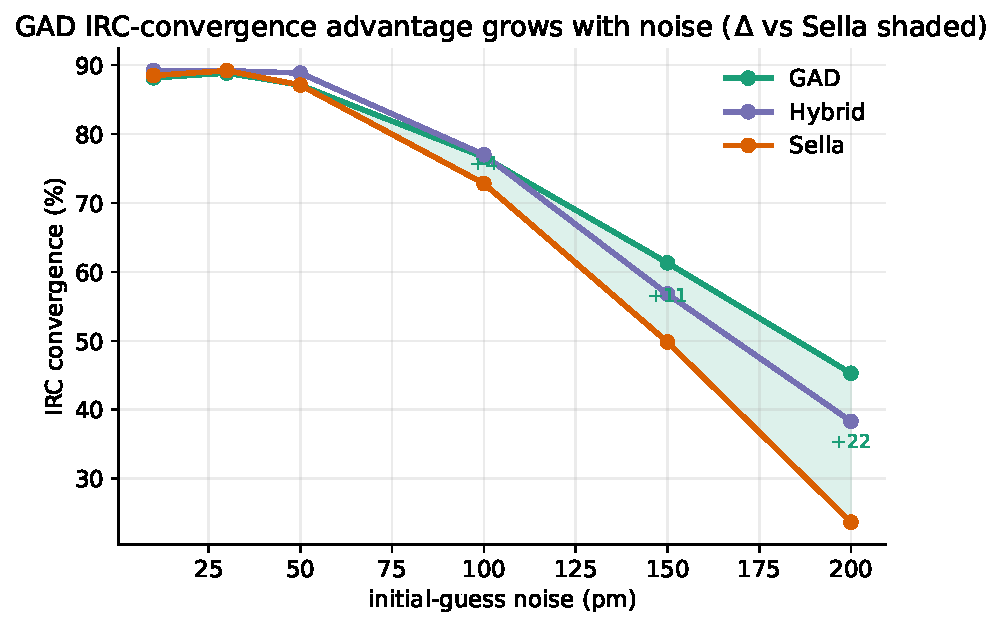
\includegraphics[width=0.66\textwidth]{figures_new/fig_intended_success_delta.pdf}
\caption{\textbf{IRC convergence for all three methods; the GAD$-$Sella gap is
shaded.} Paired-McNemar (GAD vs.\ Sella): indistinguishable
$\le\!\SI{50}{pm}$ ($p{=}1.0$), emerging at \SI{100}{pm} ($p{=}0.10$), highly
significant at \SI{150}{pm} ($p{=}3.8\!\times\!10^{-5}$) and \SI{200}{pm}
($p{=}1.7\!\times\!10^{-13}$).}
\label{fig:delta}
\end{figure}

\begin{itemize}
\item \textbf{Crossover.} Tie at low noise (intended 88--89\% at \SI{10}{pm});
  GAD pulls ahead with degradation: $\Delta$intended $=+3.9,+11.5,+21.6$~pp at
  100/150/\SI{200}{pm} (Fig.~\ref{fig:delta}, Table~\ref{tab:headline}).
\item \textbf{Significance.} McNemar on paired per-sample intended outcomes:
  n.s.\ at $\le\!\SI{50}{pm}$ ($p{=}1.0$), emerging at \SI{100}{pm} ($p{=}0.10$),
  highly significant at \SI{150}{pm} ($p{=}3.8\!\times\!10^{-5}$) and
  \SI{200}{pm} ($p{=}1.7\!\times\!10^{-13}$). The same crossover appears on
  \fmax/\nneg convergence and across \fmax{} thresholds (Section~\ref{sec:fmax}).
\end{itemize}

\begin{table}[H]\centering\small
\caption{\textbf{Primary metric --- IRC convergence rate, \%},
$n=287$, from the fresh per-sample re-validation (GAD $dt{=}0.003$); Sella $=$
strongest baseline. \fmax/\nneg convergence is reported separately in
Table~\ref{tab:conv} (Section~\ref{sec:fmax}).}
\label{tab:headline}
\begin{tabular}{l cccccc}
\toprule
\textbf{IRC convergence \%} & \textbf{10\pm} & \textbf{30\pm} & \textbf{50\pm} & \textbf{100\pm} & \textbf{150\pm} & \textbf{200\pm} \\
\midrule
GAD (ours)       & 88.2 & 88.9 & 87.1 & 76.7 & \textbf{61.3} & \textbf{45.3} \\
Sella (baseline) & 88.5 & 89.2 & 87.1 & 72.8 & 49.8 & 23.7 \\
$\Delta$ (pp)    & $-0.3$ & $-0.3$ & $0.0$ & \textbf{+3.9} & \textbf{+11.5} & \textbf{+21.6} \\
\bottomrule
\end{tabular}
\end{table}

\begin{figure}[H]\centering
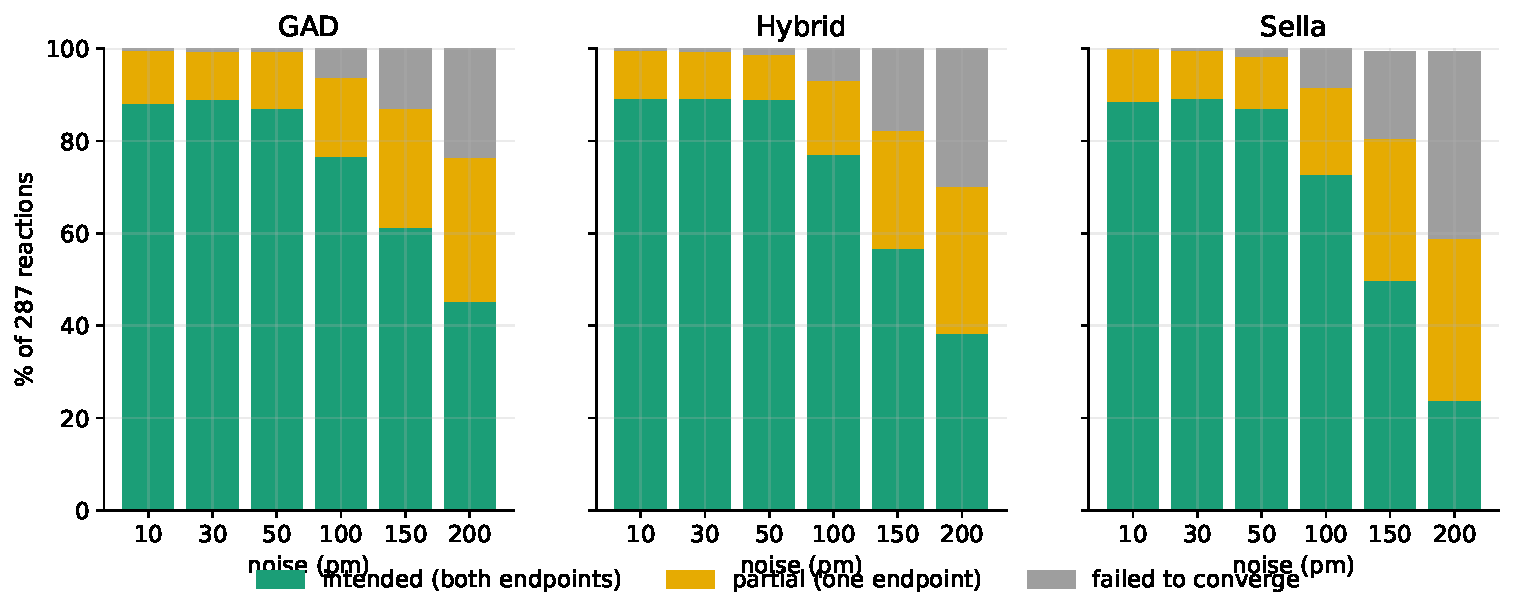
\includegraphics[width=\textwidth]{figures_new/fig_outcome_stacked.pdf}
\caption{\textbf{Full IRC outcome breakdown.} \emph{Unintended} $\approx 0$ for
every method at every noise, so the third band is purely non-convergence
(TS error / no reaction). Sella both fails to converge \emph{and} lands one-sided
(partial) saddles more often at high noise.}
\label{fig:outcome}
\end{figure}

\begin{figure}[H]\centering
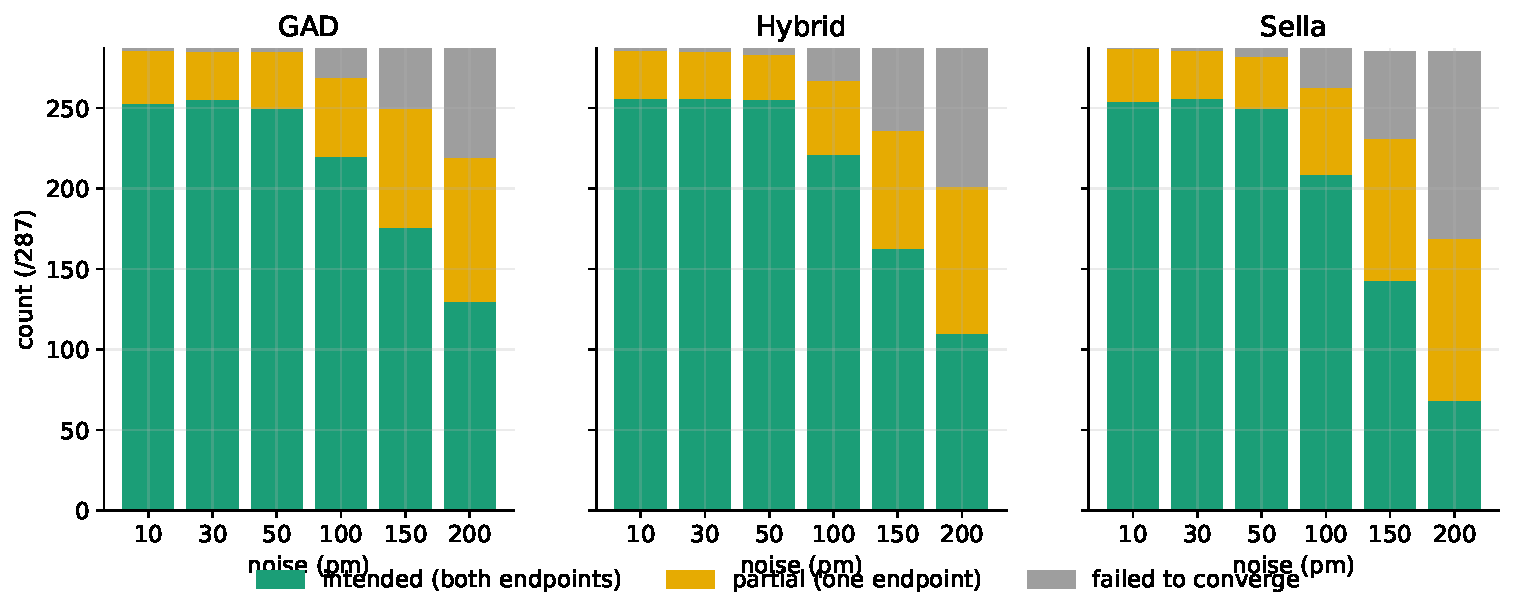
\includegraphics[width=\textwidth]{figures_new/fig_outcome_stacked_counts.pdf}
\caption{\textbf{Same breakdown, absolute counts (/287).} At \SI{200}{pm}:
intended/partial/failed $=$ GAD 130/89/68 vs.\ Sella 68/101/116 --- Sella's loss
is non-convergence (116 vs.\ 68) plus one-sided partial saddles (101 vs.\ 89).}
\label{fig:outcomecounts}
\end{figure}

\subsection{Mechanism: it is not wrong basins --- it is one-sided saddles and non-convergence}\label{sec:mech}

\begin{itemize}
\item \textbf{Unintended $\approx 0$.} The per-sample 5-tier IRC split gives
  unintended $\approx 0$ for every method at every noise: 0 for GAD and the
  hybrid, and only 2 (\SI{150}{pm}) + 2 (\SI{200}{pm}) for Sella ---
  \textbf{4 of 5166} samples total. \emph{We therefore drop the earlier ``Newton
  jumps across basin boundaries to unintended saddles'' claim --- it is
  unsupported by the data.}
\item \textbf{What actually differs} (\SI{200}{pm} illustration; whole curves in
  Fig.~\ref{fig:outcome}): intended/partial/failed $=$ \textbf{GAD 130/89/68}
  vs.\ \textbf{Sella 68/101/116}. Sella both fails to converge more \emph{and}
  lands one-sided (partial) saddles more.
\item \textbf{Why.} Small in-basin Euler steps preserve the link to \emph{both}
  reactant and product, so even non-converged GAD geometries IRC-validate on
  both sides --- intended can \emph{exceed} convergence (\SI{150}{pm}: 61.3
  vs.\ 55.1\%; \SI{200}{pm}: 45.3 vs.\ 40.8\%). Larger Newton steps more often
  drift off one channel
  ($\rightarrow$ partial) or fail to tighten ($\rightarrow$ failed).
\item \textbf{Convergence $\ne$ chemistry, stated correctly} (Fig.~\ref{fig:d1d3}):
  it is \emph{not} that convergence hides wrong saddles. (i) GAD recovers
  intended even when not strictly converged; (ii) Sella d=1 vs.\ d=3 --- d=3
  \emph{converges more} but is \emph{intended less} at every noise (a stale
  Hessian yields more partial/failed, not unintended).
\item \textbf{Non-converged GAD breakdown} (why it fails to \emph{converge}, not
  why it finds a wrong saddle): at \SI{200}{pm}, of 163 non-converged, 71 (44\%)
  drift to $\nneg\!\ge\!2$ and 92 (56\%) are plateau-orbits at $\nneg{=}1$ just
  above threshold (Section~\ref{sec:fmax}).
\end{itemize}

\begin{figure}[H]\centering
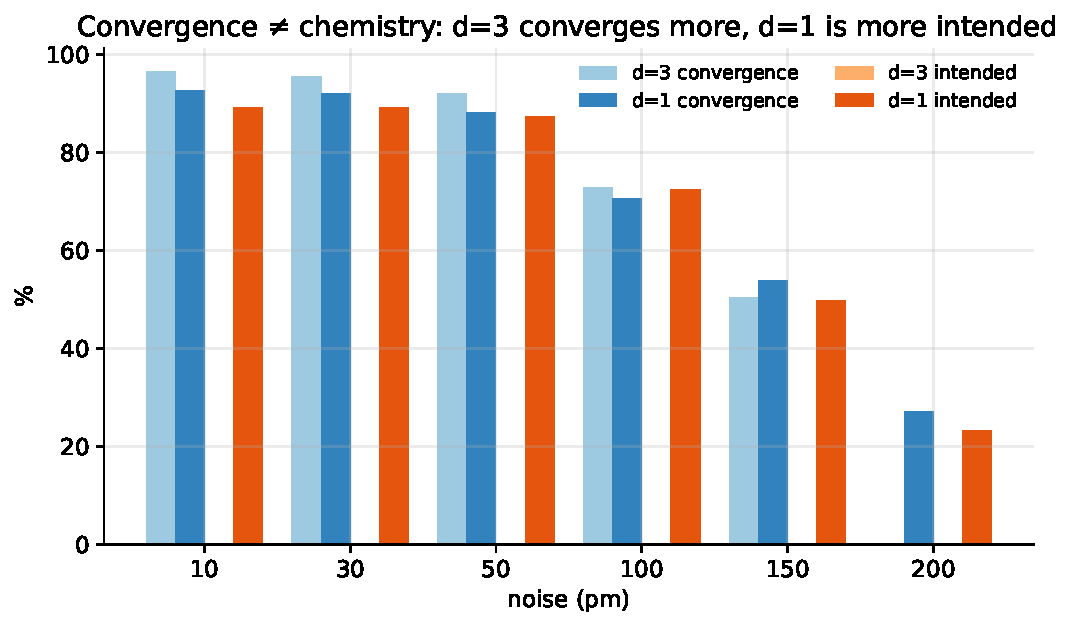
\includegraphics[width=0.82\textwidth]{figures_new/fig_d1_vs_d3.pdf}
\caption{\textbf{Convergence $\ne$ chemistry.} Sella Hess.Freq.=3 converges more
than Hess.Freq.=1 at low noise (a) yet recovers fewer intended reactions at
every noise (b): the extra ``convergences'' are one-sided (partial) saddles, not
unintended ones.}
\label{fig:d1d3}
\end{figure}

\begin{figure}[H]\centering
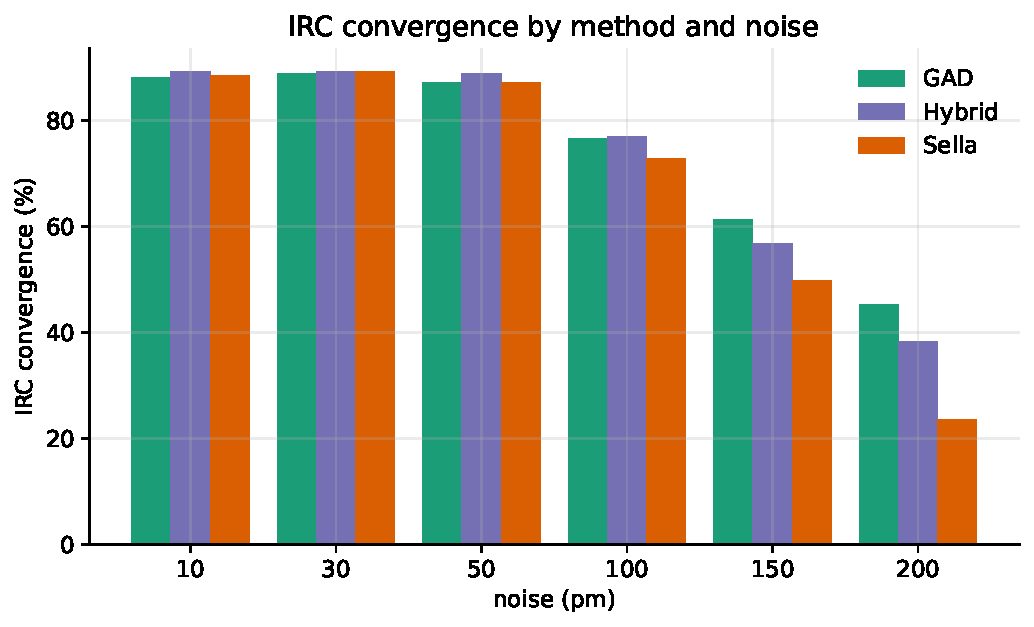
\includegraphics[width=0.78\textwidth]{figures_new/fig_outcome_grouped_intended.pdf}
\caption{\textbf{Intended reactions recovered (counts/287).} The GAD family
overtakes the baseline from \SI{100}{pm} onward.}
\label{fig:grouped}
\end{figure}

\subsection{Secondary: \texorpdfstring{$\fmax$/$\nneg$}{Fmax/nneg} convergence and the \texorpdfstring{$\fmax$}{Fmax} plateau}\label{sec:fmax}

\fmax/\nneg convergence ($\nneg{=}1 \wedge \fmax{<}\tau$) asks only whether the
optimizer reached \emph{a} first-order saddle, independent of which reaction it
connects.

\begin{itemize}
\item \textbf{Crossover here too} (Fig.~\ref{fig:conv}, Table~\ref{tab:conv}). At
  low noise Sella's Newton step crushes the force fastest, so it leads
  \fmax/\nneg convergence (92.7 vs.\ 89.2\% @ \SI{10}{pm}); GAD overtakes by
  \SI{150}{pm} (55.1 vs.\ 54.0\%) and \SI{200}{pm} (40.8 vs.\ 27.2\%).
\item \textbf{But convergence $\ne$ chemistry.} Sella's low-noise convergence
  lead does \emph{not} convert into intended reactions
  (Table~\ref{tab:headline}); the d=1/d=3 case makes this explicit
  (Fig.~\ref{fig:d1d3}).
\end{itemize}

\begin{figure}[H]\centering
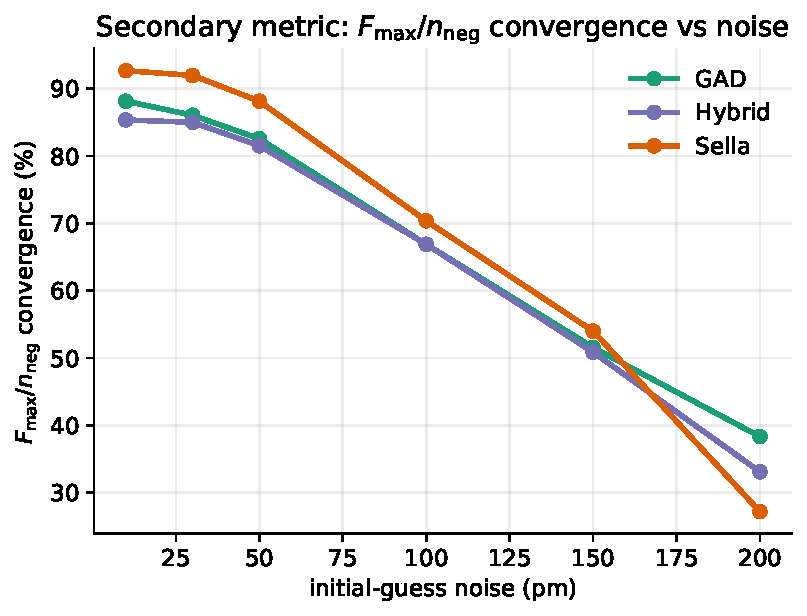
\includegraphics[width=0.6\textwidth]{figures_new/fig_saddle_convergence.pdf}
\caption{\textbf{Secondary metric: \fmax/\nneg convergence rate}
($\nneg{=}1 \wedge \fmax{<}0.01$) vs.\ noise, $n=287$. Sella leads at low noise;
GAD overtakes at high noise --- but convergence is not chemistry
(cf.\ Fig.~\ref{fig:primary}).}
\label{fig:conv}
\end{figure}

\begin{table}[H]\centering\small
\caption{\fmax/\nneg convergence rate (\%, $\nneg{=}1\wedge\fmax{<}0.01$, $n=287$).}
\label{tab:conv}
\begin{tabular}{l cccccc}
\toprule
\textbf{\fmax/\nneg convergence \%} & \textbf{10\pm} & \textbf{30\pm} & \textbf{50\pm} & \textbf{100\pm} & \textbf{150\pm} & \textbf{200\pm} \\
\midrule
GAD (ours)       & 89.2 & 88.5 & 85.4 & 71.1 & \textbf{55.1} & \textbf{40.8} \\
Sella (baseline) & \textbf{92.7} & \textbf{92.0} & \textbf{88.2} & 70.7 & 54.0 & 27.2 \\
Hybrid (ours)    & 85.4 & 85.0 & 81.5 & 66.9 & 50.9 & 33.1 \\
\bottomrule
\end{tabular}
\end{table}

\paragraph{The $\fmax$ plateau.}
\begin{itemize}
\item \textbf{Plateau.} All GAD $dt$ collapse to 0\% at $\fmax<0.005$ at every
  noise; Sella's Newton step retains 24--34\% (low noise). Pure first-order
  dynamics has no samples in \SIrange{0.001}{0.005}{eV/\AA} (Figs.~\ref{fig:plateau},
  \ref{fig:grid}).
\item \textbf{Mechanism.} GAD step $\sim dt\,\lVert\mathbf{F}\rVert$ shrinks
  linearly as $\mathbf{F}\!\to\!0$ and falls below the eigenvector noise floor;
  Newton $\sim\lVert\mathbf{H}^{-1}\mathbf{F}\rVert$ stays finite. Structural to
  fixed-step first-order dynamics; larger $dt$ trades it for instability.
\item \textbf{Intrinsic.} $5\times$ budget (10k vs.\ 2k steps, \SI{50}{pm})
  leaves $\tau{=}0.01$ unchanged (85.7\%) and $\tau{<}0.005$ exactly 0.0\%.
\item \textbf{It lives on the secondary axis.} IRC convergence
  (Section~\ref{sec:primary}) needs no sub-plateau force, so the plateau does
  not affect the primary metric.
\end{itemize}

\begin{figure}[H]\centering
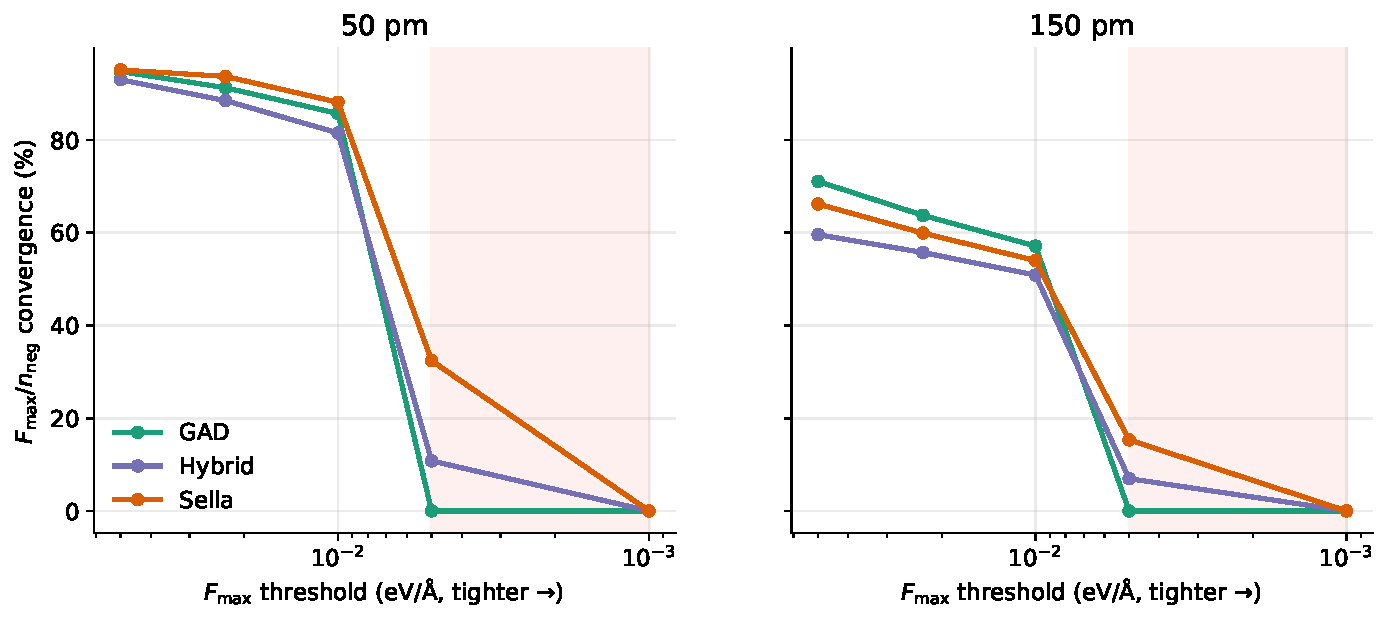
\includegraphics[width=0.92\textwidth]{figures_new/fig_fmax_plateau.pdf}
\caption{\textbf{The $\fmax$ plateau (50 and \SI{150}{pm} noise).}
\fmax/\nneg convergence rate (\%, $y$) vs.\ the $\fmax$ threshold ($x$, log axis,
tightening to the right; shaded $=$ the sub-$0.005$ plateau zone), one line per
method. GAD drops vertically near $\fmax{=}0.01$ --- it has essentially no
converged samples below it --- whereas Sella and the hybrid keep descending into
the $0.005$ band because their trust-radius-capped Newton step continues to drive
the residual force down. No method reaches $0.001$ within the 2{,}000-step budget.}
\label{fig:plateau}
\end{figure}

\begin{figure}[H]\centering
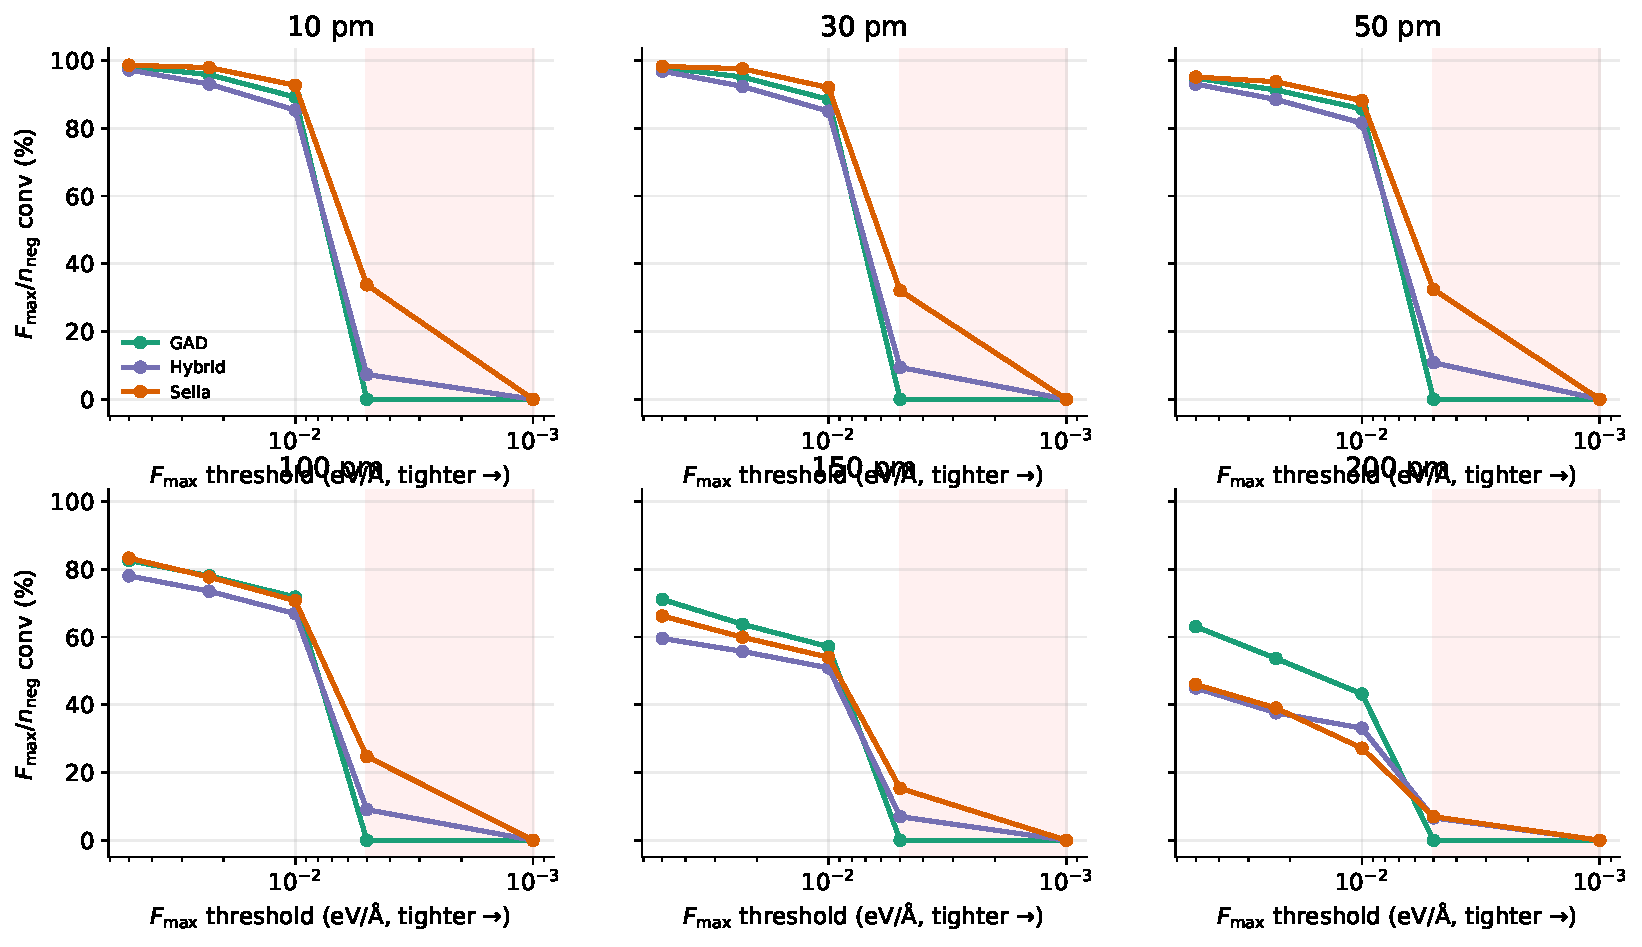
\includegraphics[width=0.95\textwidth]{figures_new/fig_fmax_plateau_grid.pdf}
\caption{\textbf{\fmax/\nneg convergence vs.\ $\fmax$ threshold, one panel per noise
level (10--\SI{200}{pm}).} Each panel plots convergence rate (\%) against the
force threshold (log $x$, tightening to the right; shaded $=$ plateau zone) for
GAD, the hybrid, and the Sella baseline. The GAD curve collapses vertically to
0\% at $\fmax<0.005$ in \emph{every} panel, whereas Sella and the hybrid descend
further --- the plateau is a property of the fixed-step first-order dynamics,
universal across noise.}
\label{fig:grid}
\end{figure}

\subsection{Cost and geometry: the hybrid wins both}\label{sec:cost}

\begin{itemize}
\item \textbf{Wall-time / converged TS:} hybrid lowest at every noise ---
  $1.3$--$3.0\times$ vs.\ Sella, $3.6$--$4.5\times$ vs.\ GAD (Fig.~\ref{fig:wall},
  Table~\ref{tab:cost}). Few-but-expensive Sella steps (4--13) vs.\
  many-cheap GAD steps (100--738) vs.\ intermediate-cheap hybrid (6--95)
  (Fig.~\ref{fig:steps}). Pareto-dominant at high noise (Fig.~\ref{fig:pareto}).
\item \textbf{Geometry:} converged-TS RMSD-to-reference --- hybrid holds the
  tightest p95 at high noise (\SI{200}{pm}: \textbf{0.109} vs.\ GAD 0.456 vs.\
  Sella 0.838~\AA; $7.7\times$ tighter than Sella). Sella's tail is bimodal
  (Fig.~\ref{fig:rmsd}, Table~\ref{tab:rmsd}).
\end{itemize}

\begin{figure}[H]\centering
\begin{minipage}{0.49\textwidth}\centering
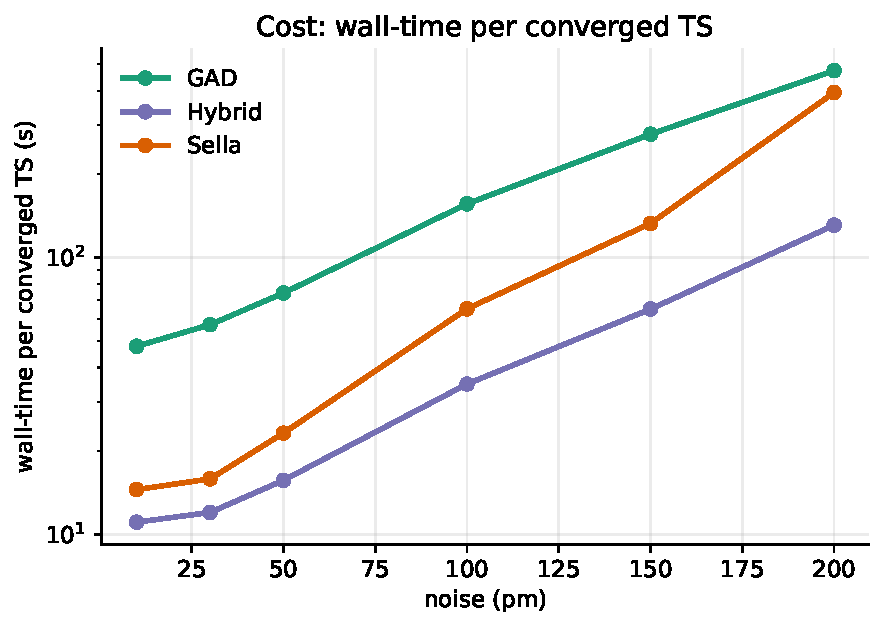
\includegraphics[width=\textwidth]{figures_new/fig_walltime.pdf}\end{minipage}\hfill
\begin{minipage}{0.49\textwidth}\centering
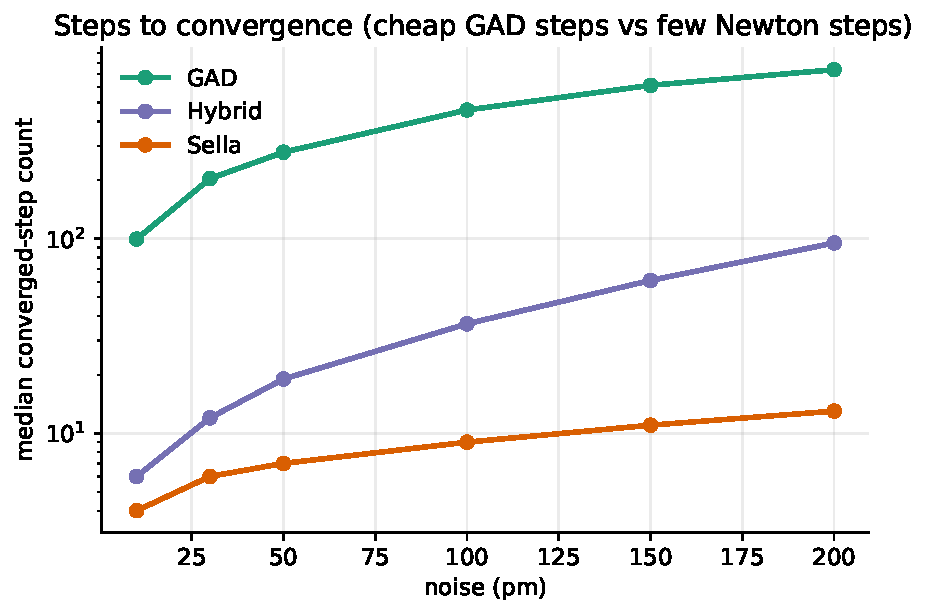
\includegraphics[width=\textwidth]{figures_new/fig_steps.pdf}\end{minipage}
\caption{\textbf{Cost.} Wall-time per converged TS (left) and median steps
(right). The hybrid is fastest despite more steps than Sella, because its steps
are cheap.}
\label{fig:wall}\label{fig:steps}
\end{figure}

\begin{figure}[H]\centering
\begin{minipage}{0.46\textwidth}\centering
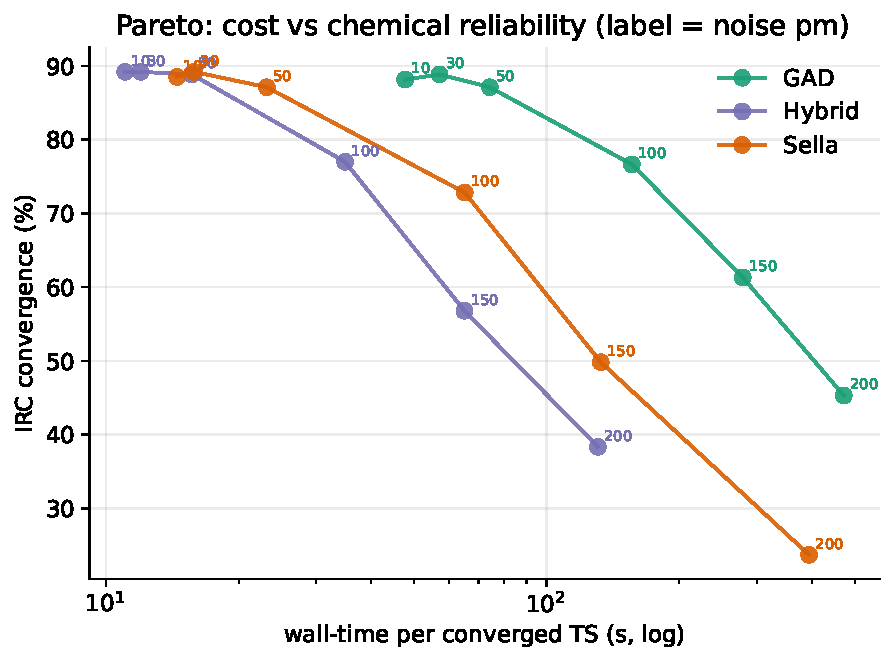
\includegraphics[width=\textwidth]{figures_new/fig_pareto.pdf}\end{minipage}\hfill
\begin{minipage}{0.52\textwidth}\centering
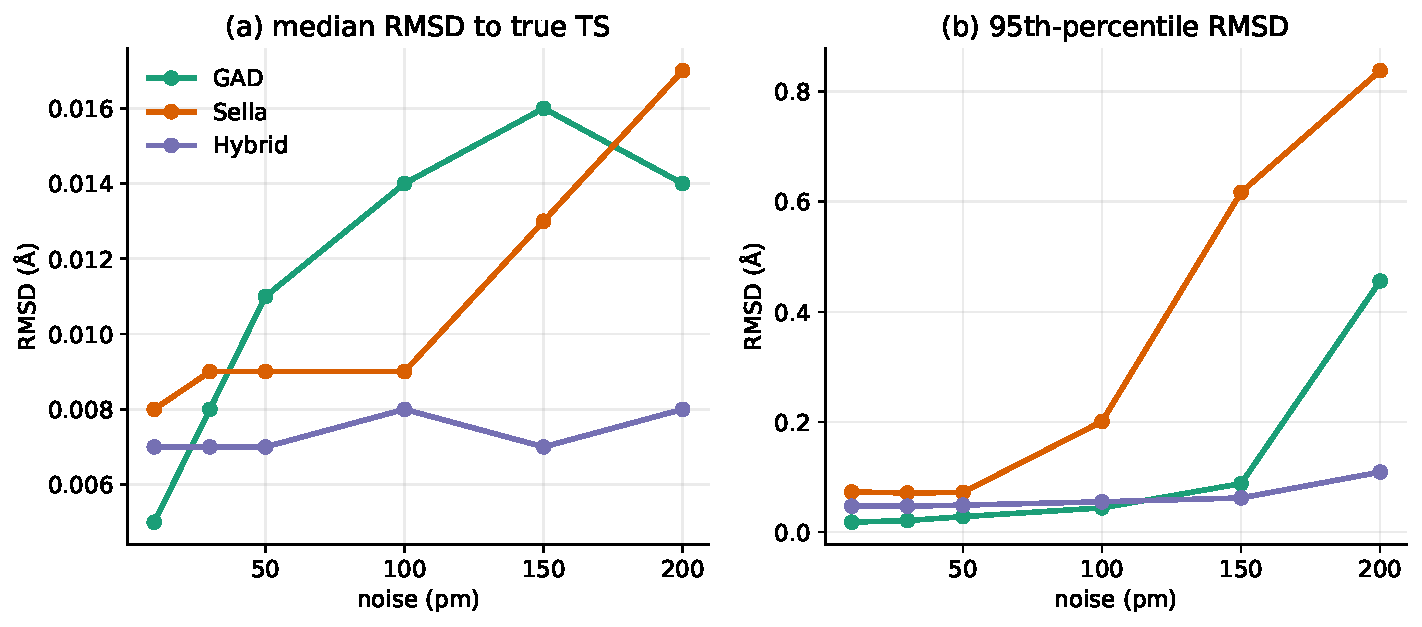
\includegraphics[width=\textwidth]{figures_new/fig_rmsd_vs_noise.pdf}\end{minipage}
\caption{\textbf{Left: Pareto} (intended vs.\ wall-time; up-left is better) ---
the hybrid is dominant at high noise. \textbf{Right: RMSD to true TS} (median and
p95) --- the hybrid holds the tightest tail.}
\label{fig:pareto}\label{fig:rmsd}
\end{figure}

\begin{table}[H]\centering\small
\caption{Wall-time per converged TS (s) and converged-TS RMSD (\AA, p95),
$\fmax<0.01$, $n=287$.}
\label{tab:cost}\label{tab:rmsd}
\begin{tabular}{ll cccccc}
\toprule
& & \textbf{10\pm} & \textbf{30\pm} & \textbf{50\pm} & \textbf{100\pm} & \textbf{150\pm} & \textbf{200\pm} \\
\midrule
\multirow{3}{*}{\textbf{wall/conv (s)}}
 & \textbf{Hybrid} & \textbf{11.0} & \textbf{12.0} & \textbf{15.7} & \textbf{34.9} & \textbf{65.0} & \textbf{130.7} \\
 & Sella           & 14.5 & 15.8 & 23.2 & 65.2 & 132.6 & 393.8 \\
 & GAD             & 47.7 & 57.1 & 74.3 & 156.0 & 278.5 & 472.3 \\
\midrule
\multirow{3}{*}{\textbf{p95 RMSD (\AA)}}
 & \textbf{Hybrid} & 0.047 & 0.047 & 0.049 & \textbf{0.055} & \textbf{0.062} & \textbf{0.109} \\
 & Sella           & 0.073 & 0.071 & 0.072 & 0.201 & 0.617 & 0.838 \\
 & GAD             & 0.018 & 0.021 & 0.028 & 0.044 & 0.088 & 0.456 \\
\bottomrule
\end{tabular}
\end{table}

\subsection{Scope boundary: GAD needs to start near the saddle}\label{sec:scope}

\begin{itemize}
\item Robustness above is for \emph{perturbed-saddle} guesses. From a
  \emph{reactant} start the GAD family is weak: hybrid $\sim$\textbf{2\%},
  GAD $dt{=}0.005$ 54\% (partial $n$), while Sella reaches 81\%
  (Fig.~\ref{fig:scope}).
\item Interpretation: far from the saddle the reaction mode is not yet
  identifiable as the lowest Eckart-projected eigenvector, so the GAD reflection
  has no correct direction to climb. GAD/hybrid are TS \emph{refiners} given a
  near-saddle guess, not single-ended searchers from a minimum.
\end{itemize}

\begin{figure}[H]\centering
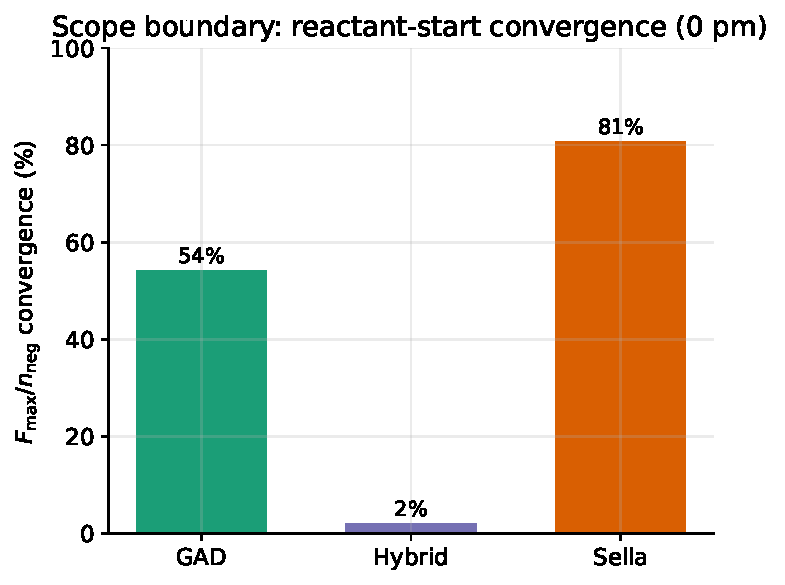
\includegraphics[width=0.52\textwidth]{figures_new/fig_reactant_scope.pdf}
\caption{\textbf{Scope boundary.} Convergence from a reactant start: Sella wins;
the GAD family needs a near-saddle guess.}
\label{fig:scope}
\end{figure}

% =====================================================================
\section{Discussion}
% =====================================================================
\begin{itemize}
\item When the analytic Hessian is cheap, the limiting factor is the step, not
  the curvature budget. A minimal first-order GAD walk is more robust on the
  metric that matters (IRC convergence) precisely where large Newton/RFO jumps
  fail --- under a degraded guess --- while tying at low noise.
\item The failure is \emph{not} wrong basins: across all methods, converged
  geometries essentially never connect the wrong reaction. The high-noise gap is
  non-convergence plus one-sided (partial) saddles, which the small in-basin
  Euler step avoids.
\item \textbf{Recommended default:} Hybrid GAD--Newton --- fastest per converged
  TS, geometrically tightest, and chemically as reliable as GAD --- for
  near-saddle (refinement) guesses.
\item \textbf{Limitations:} (i) demonstrated for perturbed-saddle guesses; from a
  reactant start the GAD family is weak and Sella wins (Section~\ref{sec:scope}).
  (ii) Convergence below $\tau{=}0.001$ is unreachable for all methods here.
  (iii) Isotropic perturbations; template/interpolation guesses carry structured
  error (future work).
\end{itemize}

\appendix
\section*{\large Appendix}
\addcontentsline{toc}{section}{Appendix}

\section{Full tables (all nine configurations, $\fmax<0.01$, $n=287$)}\label{app:fulltables}
\begin{table}[H]\centering\footnotesize
\caption{Intended-reaction success \% (top) and \fmax/\nneg convergence \% (bottom), all
nine configurations, from the aggregate IRC sweep. Bold = column best. The three
headline methods (GAD, Sella cart+Eckart untuned d=1, Hybrid damped) were
independently re-validated per-sample (\texttt{FINDING\_IRC\_5TIER\_2026\_06\_23};
\texttt{irc\_outcomes\_5tier\_test287.csv}); main-text numbers use that fresh
re-validation and differ here by $\le$2~pp, with unintended $\approx 0$ confirmed.}
\begin{tabular}{l cccccc}
\toprule
\textbf{Intended \%} & \textbf{10\pm} & \textbf{30\pm} & \textbf{50\pm} & \textbf{100\pm} & \textbf{150\pm} & \textbf{200\pm} \\
\midrule
GAD $dt=0.003$ & 88.5 & \textbf{89.2} & \textbf{88.9} & \textbf{78.4} & 61.0 & \textbf{44.6} \\
GAD $dt=0.005$ & 88.9 & \textbf{89.2} & \textbf{88.9} & 78.0 & \textbf{61.7} & \textbf{44.6} \\
GAD $dt=0.007$ & 88.5 & 88.5 & 88.5 & \textbf{78.4} & \textbf{61.7} & 43.9 \\
Sella cart tuned d=1          & 88.9 & 88.9 & 87.5 & 70.7 & 46.7 & 17.8 \\
Sella cart+Eck untuned d=1    & \textbf{89.2} & \textbf{89.2} & 87.5 & 72.5 & 49.8 & 23.3 \\
Sella internal tuned d=1      & 88.2 & 87.5 & 83.3 & 64.5 & 33.1 & 16.0 \\
Sella cart+Eck untuned d=3    & 88.5 & 88.9 & 87.1 & 70.4 & 45.3 & 22.0 \\
Hybrid damped Eckart tr=0.05  & \textbf{89.2} & 88.9 & \textbf{88.9} & 76.7 & 57.5 & 38.7 \\
Hybrid undamped Eckart tr=0.05& 88.9 & 88.9 & 88.5 & 77.0 & 57.1 & 38.7 \\
\midrule
\textbf{\fmax/\nneg convergence \%} & & & & & & \\
\midrule
GAD $dt=0.003$ & 89.2 & 88.5 & 85.4 & 71.1 & 55.1 & 40.8 \\
GAD $dt=0.005$ & 89.2 & 88.5 & 85.7 & 71.8 & 57.1 & 43.2 \\
GAD $dt=0.007$ & 89.2 & 88.9 & 85.7 & \textbf{72.8} & \textbf{58.2} & \textbf{44.6} \\
Sella cart tuned d=1          & 92.0 & 91.3 & 87.5 & 65.5 & 42.9 & 18.8 \\
Sella cart+Eck untuned d=1    & 92.7 & 92.0 & 88.2 & 70.7 & 54.0 & 27.2 \\
Sella internal tuned d=1      & 79.1 & 77.4 & 71.8 & 50.9 & 26.8 & 13.9 \\
Sella cart+Eck untuned d=3    & \textbf{96.5} & \textbf{95.5} & \textbf{92.0} & \textbf{72.8} & 50.5 & 23.3 \\
Hybrid damped Eckart tr=0.05  & 85.4 & 85.0 & 81.5 & 66.9 & 50.9 & 33.1 \\
Hybrid undamped Eckart tr=0.05& 84.7 & 84.3 & 81.5 & 65.5 & 49.8 & 31.0 \\
\bottomrule
\end{tabular}
\end{table}

\section{Comprehensive \texorpdfstring{$\fmax$}{Fmax} sweep (convergence \%, $n=287$)}\label{app:fmaxtable}
\begin{table}[H]\centering\footnotesize
\caption{Convergence at five thresholds; GAD block is 0.0\% at $\fmax<0.005$ everywhere.}
\begin{tabular}{ll cccccc}
\toprule
\textbf{thr} & \textbf{method} & \textbf{10\pm} & \textbf{30\pm} & \textbf{50\pm} & \textbf{100\pm} & \textbf{150\pm} & \textbf{200\pm} \\
\midrule
\multirow{3}{*}{0.05}
 & GAD $dt{=}0.005$ & 98.3 & 97.9 & 94.8 & 82.6 & 71.1 & 63.1 \\
 & Sella d=1        & 98.6 & 98.3 & 95.1 & 83.3 & 66.2 & 46.0 \\
 & Hybrid damped    & 97.2 & 96.9 & 93.0 & 78.0 & 59.6 & 44.9 \\
\midrule
\multirow{3}{*}{0.01}
 & GAD $dt{=}0.005$ & 89.2 & 88.5 & 85.7 & 71.8 & 57.1 & 43.2 \\
 & Sella d=1        & 92.7 & 92.0 & 88.2 & 70.7 & 54.0 & 27.2 \\
 & Hybrid damped    & 85.4 & 85.0 & 81.5 & 66.9 & 50.9 & 33.1 \\
\midrule
\multirow{3}{*}{0.005}
 & GAD $dt{=}0.005$ & \textbf{0.0} & \textbf{0.0} & \textbf{0.0} & \textbf{0.0} & \textbf{0.0} & \textbf{0.0} \\
 & Sella d=1        & 33.8 & 32.1 & 32.4 & 24.7 & 15.3 & 7.0 \\
 & Hybrid damped    & 7.3 & 9.4 & 10.8 & 9.1 & 7.0 & 6.6 \\
\bottomrule
\end{tabular}
\end{table}

\section{Convergence-criterion family}\label{app:crit}
Force thresholds (\si{eV/\AA}): ASE default 0.05; Gaussian ``Normal'' max-force
0.0231 ($4.50\!\times\!10^{-4}E_h/a_0$); project canonical 0.01; tight 0.005;
Sella documentation 0.001. \fmax{} = maximum force component on any atom.

\section{Sella baseline configurations}\label{app:sella}
Three axes: \textbf{\{cartesian$|$internal\} \{Eckart\}? \{tuned$|$untuned\}
Hess.Freq.=$N$}. Headline baseline: cartesian + Eckart, untuned, Hess.Freq.=1
(exact Hessian every step). Hess.Freq.=3 (library default) raises convergence at
low noise (96.5 vs.\ 92.7\% @ \SI{10}{pm}) but lowers IRC convergence at every
noise (Fig.~\ref{fig:d1d3}) --- a stale Hessian yields more one-sided/failed
outcomes, not unintended ones.

\section{Reproducibility}\label{app:repro}
{\sloppy
\begin{itemize}
\item \textbf{Data (committed CSVs):} \texttt{master\_2026\_05\_16.csv},
  \texttt{noise\_sweep\_with\_irc.csv}, \texttt{irc\_topo\_existing\_methods.csv},
  \texttt{irc\_topo\_hybrid.csv}, \texttt{threshold\_sweep\_2026\_05\_16.csv},
  \texttt{rmsd\_to\_known\_ts\_compare.csv}, \texttt{reactant\_0pm\_2026\_05\_16.csv},
  \texttt{test\_summary\_full.csv} (per-sample).
\item \textbf{Figures:} \texttt{make\_figs2.py}. \textbf{Code:} \texttt{core/gad.py}
  (Eq.~\ref{eq:gad}), \texttt{projection/projection.py},
  \texttt{search/hybrid\_gad\_eigfollownewton\_eckart.py},
  \texttt{search/irc\_validate.py} (Sella IRC + VF2).
\item Headline numbers are full $n=287$. The \SI{200}{pm} count illustration
  (130/89/68; 68/101/116) is from the latest local re-scoring and may differ by a
  few counts from the committed aggregate CSVs; McNemar significance is from the
  per-sample paired analysis.
\end{itemize}
\par}

\begin{thebibliography}{99}\small
\bibitem{gad} W.~E and X.~Zhou, \emph{Nonlinearity} \textbf{24}, 1831 (2011).
\bibitem{dimer} G.~Henkelman and H.~J\'onsson, \emph{J. Chem. Phys.} \textbf{111}, 7010 (1999).
\bibitem{cerjanmiller} C.~J.~Cerjan and W.~H.~Miller, \emph{J. Chem. Phys.} \textbf{75}, 2800 (1981).
\bibitem{banerjee} A.~Banerjee, N.~Adams, J.~Simons, R.~Shepard, \emph{J. Phys. Chem.} \textbf{89}, 52 (1985).
\bibitem{baker} J.~Baker, \emph{J. Comput. Chem.} \textbf{7}, 385 (1986).
\bibitem{sella2019} E.~D.~Hermes, K.~Sargsyan, H.~N.~Najm, J.~Z\'ador, \emph{J. Chem. Theory Comput.} \textbf{15}, 6536 (2019).
\bibitem{sella2022} E.~D.~Hermes, K.~Sargsyan, H.~N.~Najm, J.~Z\'ador, \emph{J. Chem. Theory Comput.} \textbf{18}, 6974 (2022).
\bibitem{transition1x} M.~Schreiner, A.~Bhowmik, T.~Vegge, J.~Busk, O.~Winther, \emph{Sci. Data} \textbf{9}, 779 (2022).
\bibitem{hip} A.~Burger, L.~Thiede, N.~R{\o}nne, \emph{et al.}, ``Shoot from the HIP: Hessian interatomic potentials without derivatives,'' arXiv:2509.21624 (2025).
\bibitem{newtonnet} E.~C.-Y.~Yuan, \emph{et al.}, \emph{Nat. Commun.} \textbf{15}, 8865 (2024); arXiv:2405.02247.
\bibitem{lmhe} G.~Wu, C.-Y.~Yuan, K.~Hegazy, S.~M.~Blau, T.~Head-Gordon, arXiv:2603.21323 (2026).
\end{thebibliography}


% =====================================================================
\clearpage
\section{Figure gallery (one joint view per result)}\label{app:gallery}
One curated figure per result, favouring the joint multi-panel / multi-line views. Sources: \texttt{figures\_new/} (fresh test-287 5-tier IRC, built by \texttt{scripts/build\_figures\_new.py}) and \texttt{figures/fig\_master\_4axis} (all-method comparison).

\begin{figure}[htbp]\centering
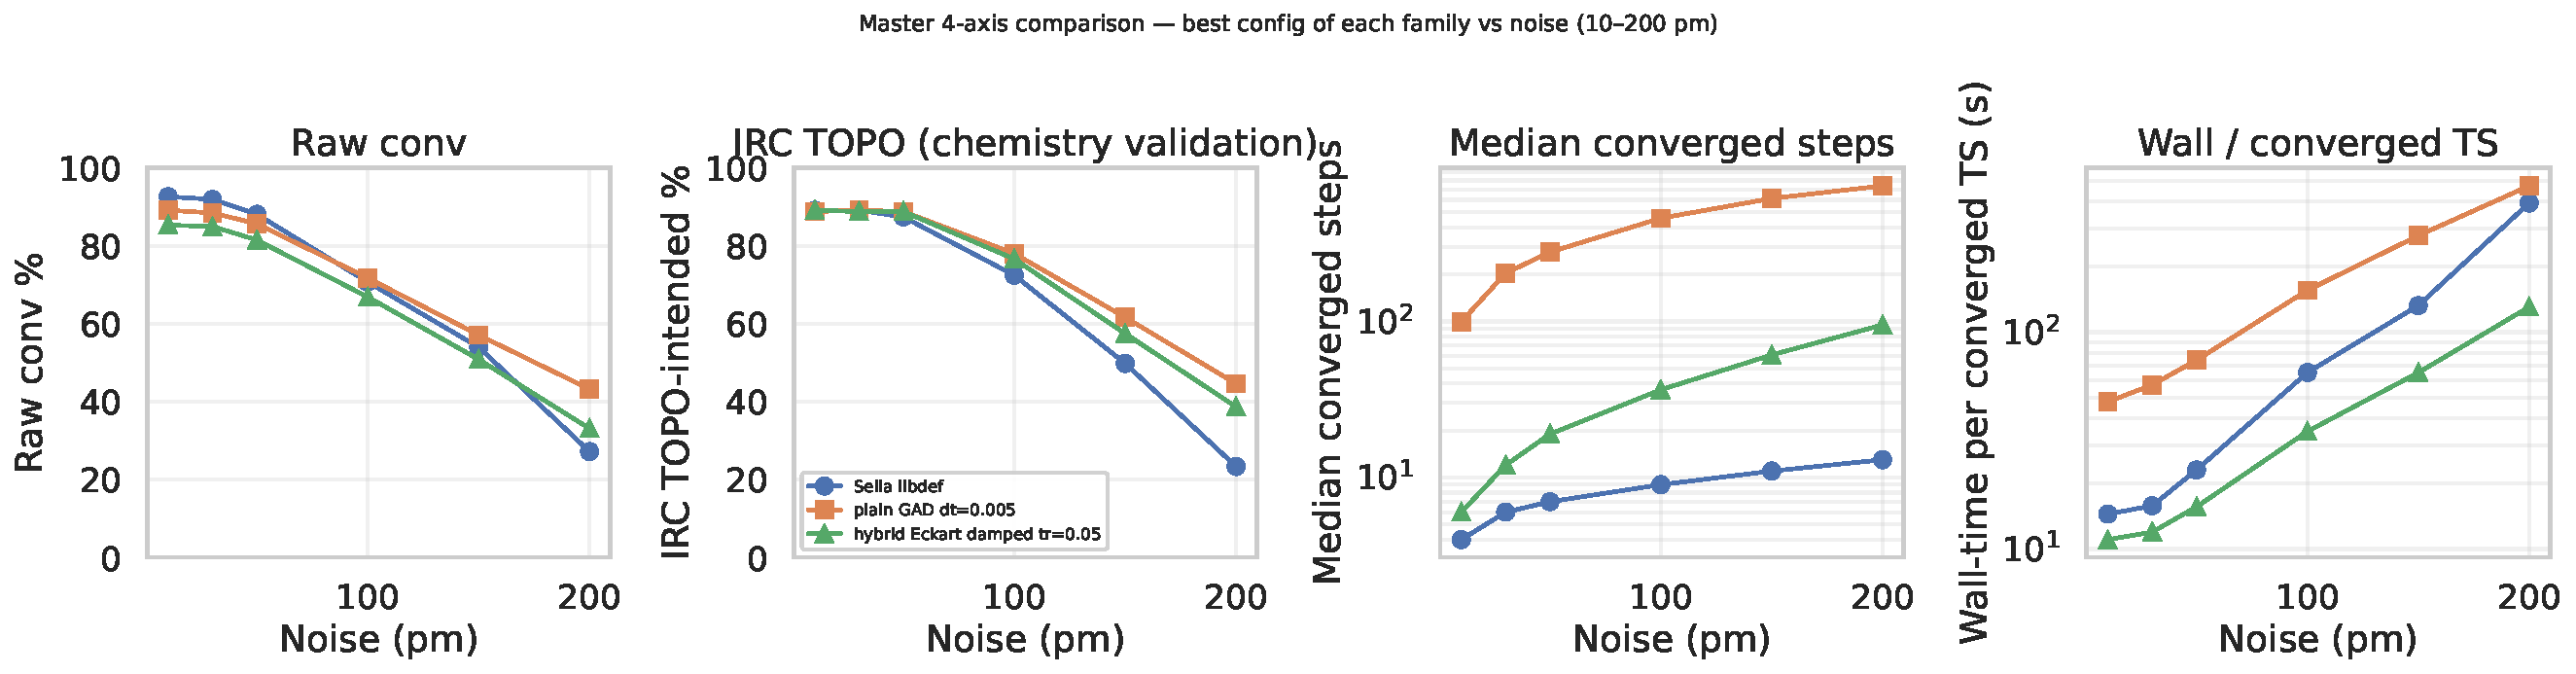
\includegraphics[width=0.95\textwidth,height=0.42\textheight,keepaspectratio]{figures/fig_master_4axis.pdf}
\caption{\textbf{All-method four-axis summary (joint).} Intended-reaction success, \fmax/\nneg convergence, wall-time per converged TS, and RMSD-to-true-TS, all nine configurations plotted against initial-guess noise on one set of axes ($n=287$). The single most complete view of the benchmark.}
\label{fig:gal0}
\end{figure}
\begin{figure}[htbp]\centering
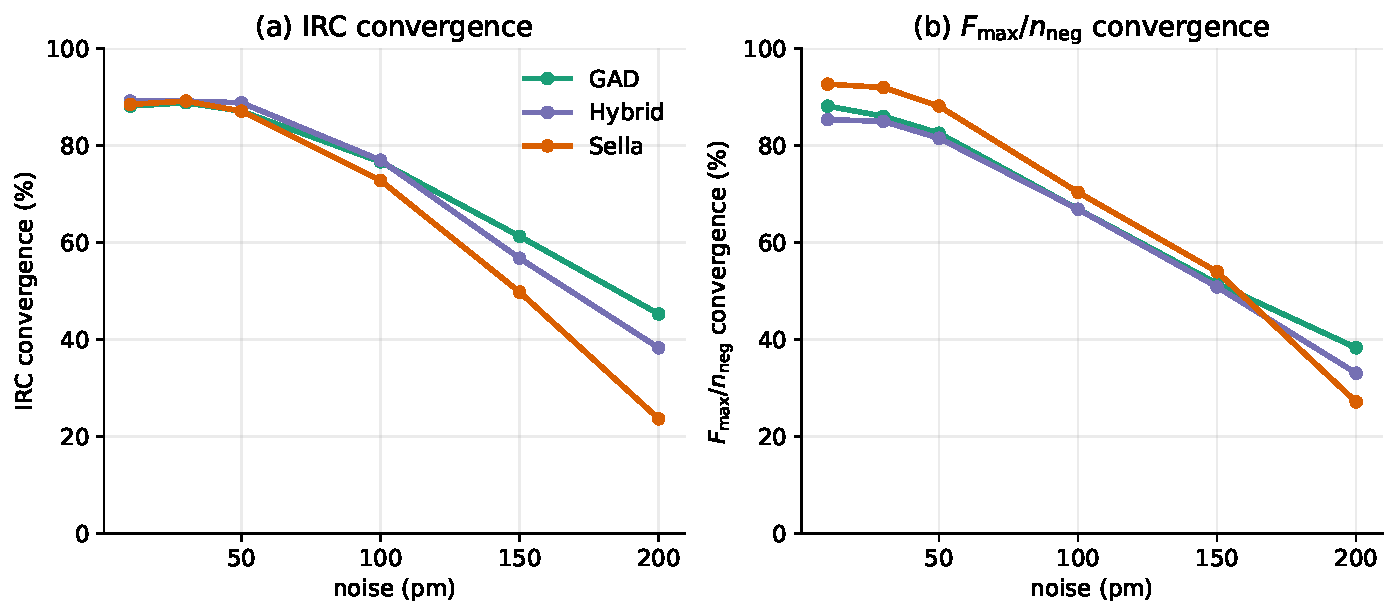
\includegraphics[width=\textwidth,height=0.42\textheight,keepaspectratio]{figures_new/fig_intended_success.pdf}
\caption{\textbf{Primary result (focused).} Intended-reaction success (left) and \fmax/\nneg convergence (right) vs.\ noise for GAD, the hybrid, and the strongest Sella baseline. The methods tie when the guess is good and GAD pulls ahead as it degrades; the crossover holds on both axes.}
\label{fig:gal1}
\end{figure}
\clearpage
\begin{figure}[htbp]\centering
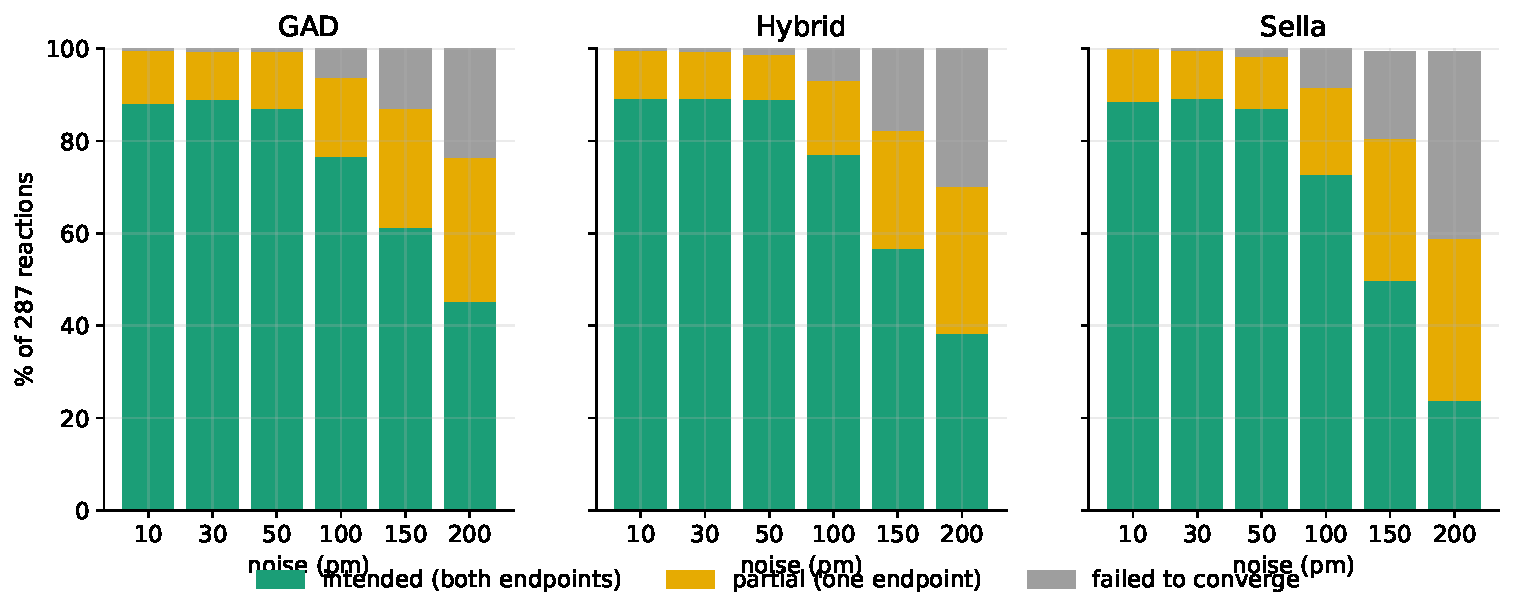
\includegraphics[width=\textwidth,height=0.42\textheight,keepaspectratio]{figures_new/fig_outcome_stacked.pdf}
\caption{\textbf{IRC outcome composition.} Each bar splits the 287 reactions into intended, partial (one-sided), and failed-to-converge. No method produces \emph{unintended} saddles; the high-noise gap is one-sided recovery plus non-convergence, not wrong basins.}
\label{fig:gal2}
\end{figure}
\begin{figure}[htbp]\centering
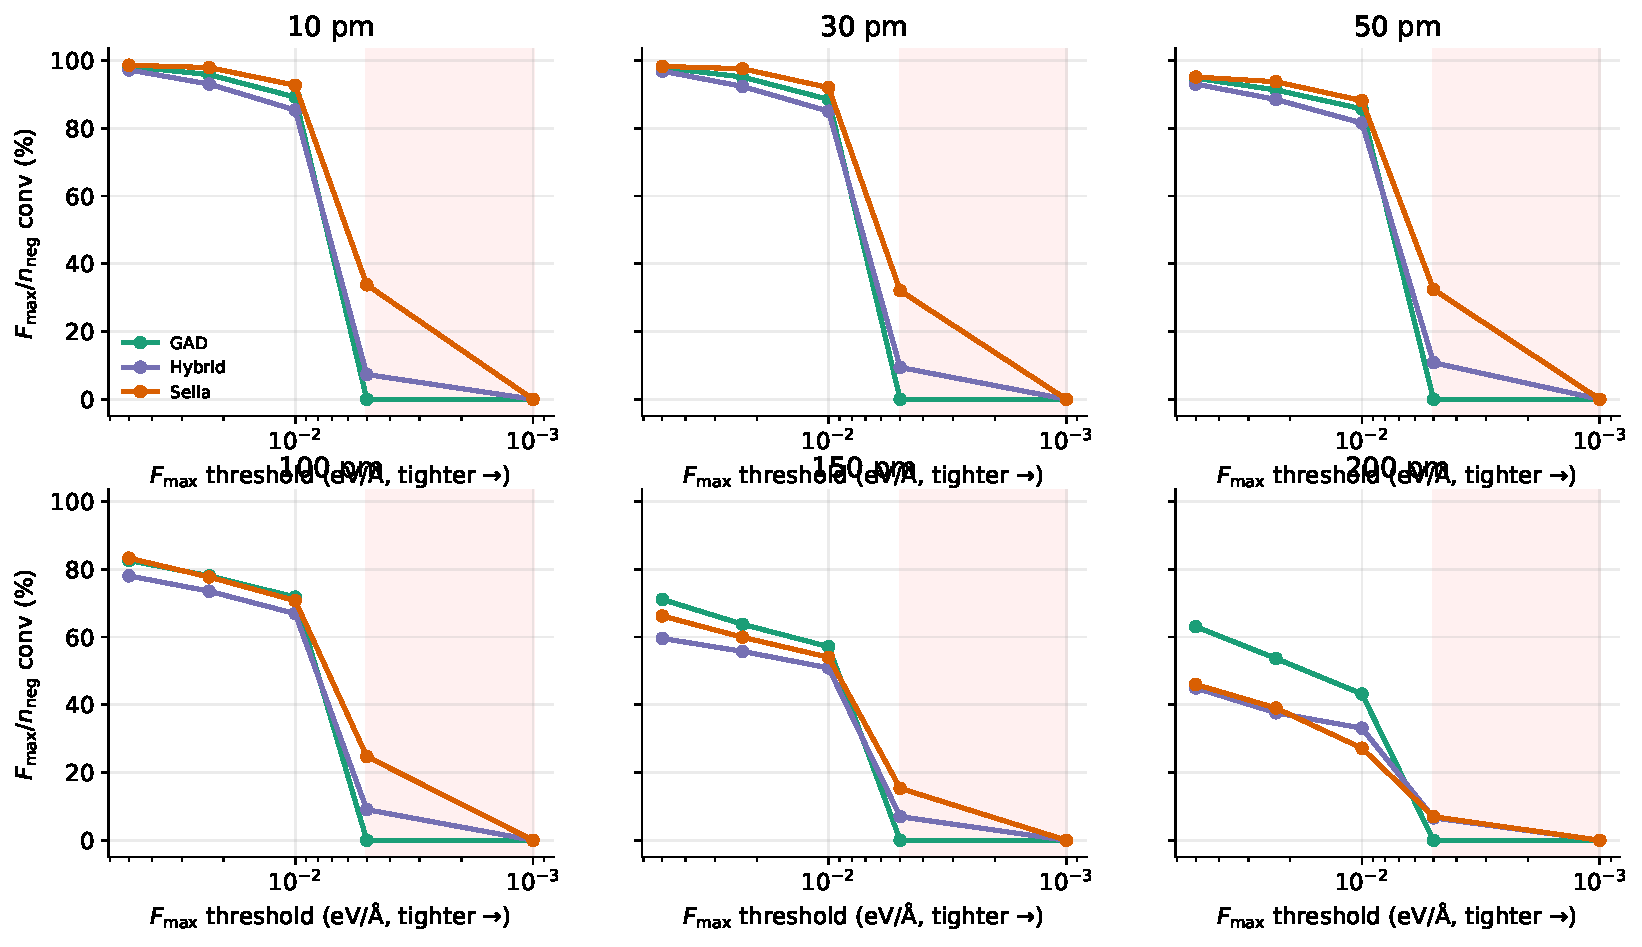
\includegraphics[width=0.95\textwidth,height=0.42\textheight,keepaspectratio]{figures_new/fig_fmax_plateau_grid.pdf}
\caption{\textbf{The $F_\mathrm{max}$ plateau across all noise levels.} Convergence vs.\ force threshold; GAD cliffs to zero below $\approx\!0.01$~eV/\AA{} at every noise level while the Newton-based methods descend further.}
\label{fig:gal3}
\end{figure}
\clearpage
\begin{figure}[htbp]\centering
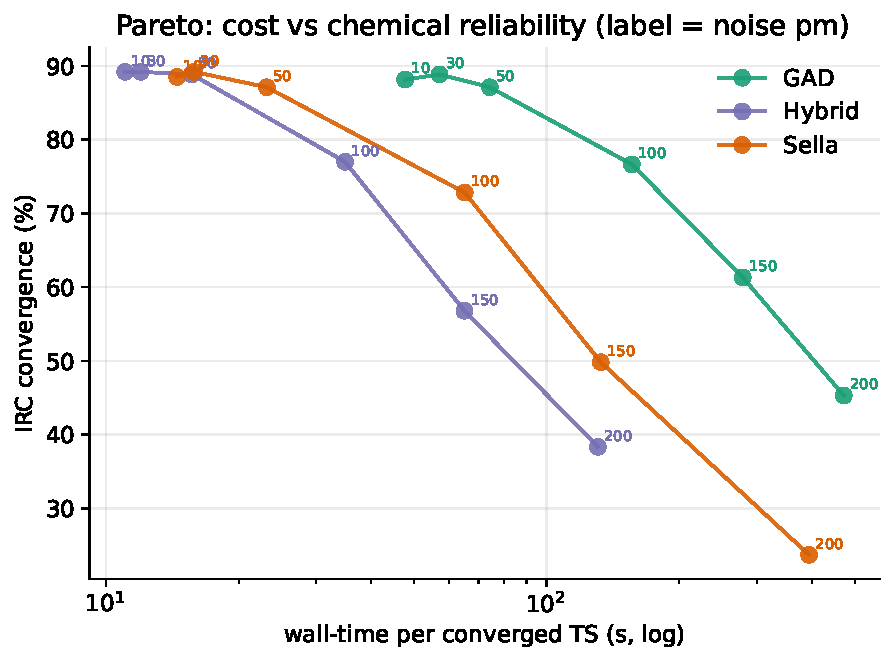
\includegraphics[width=0.72\textwidth,height=0.42\textheight,keepaspectratio]{figures_new/fig_pareto.pdf}
\caption{\textbf{Cost vs.\ chemical reliability (joint).} Wall-time per converged TS against IRC convergence, one point per noise level per method. The hybrid is Pareto-dominant at high noise.}
\label{fig:gal4}
\end{figure}
\begin{figure}[htbp]\centering
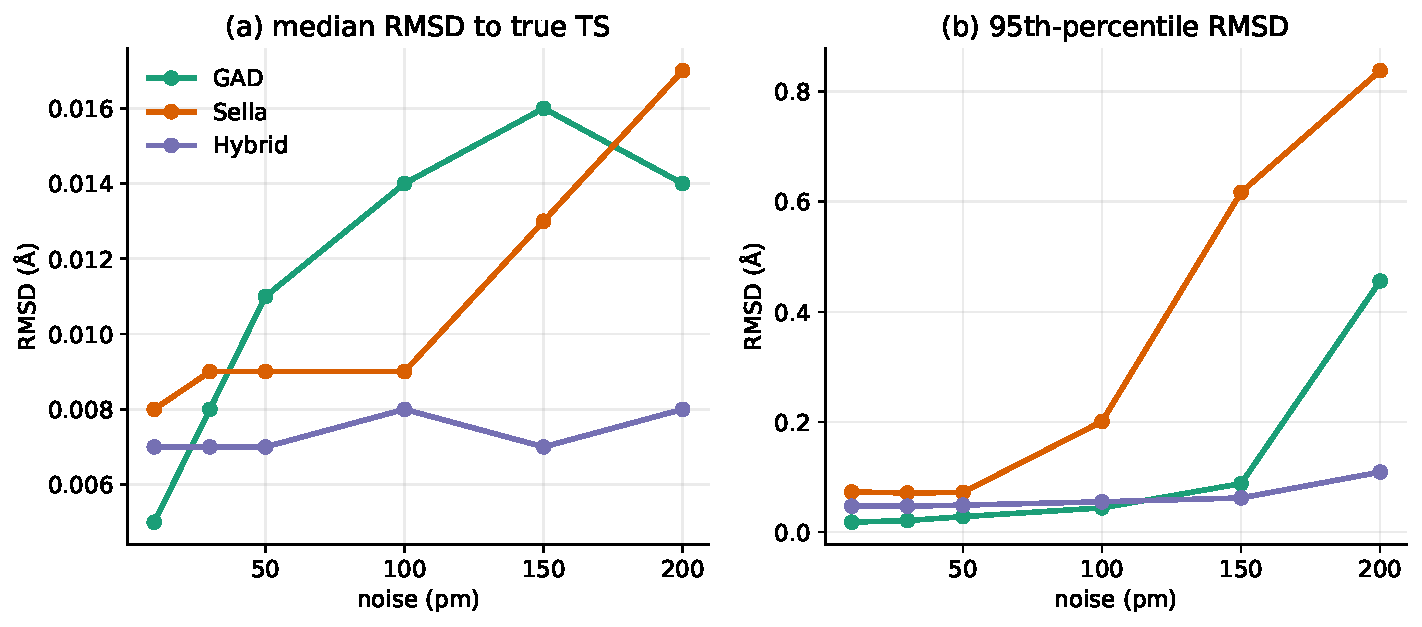
\includegraphics[width=0.72\textwidth,height=0.42\textheight,keepaspectratio]{figures_new/fig_rmsd_vs_noise.pdf}
\caption{\textbf{Geometric quality.} Median and 95th-percentile RMSD of the converged TS to the labelled saddle vs.\ noise; the hybrid stays tight where Sella develops a large-RMSD tail.}
\label{fig:gal5}
\end{figure}
\clearpage
\begin{figure}[htbp]\centering
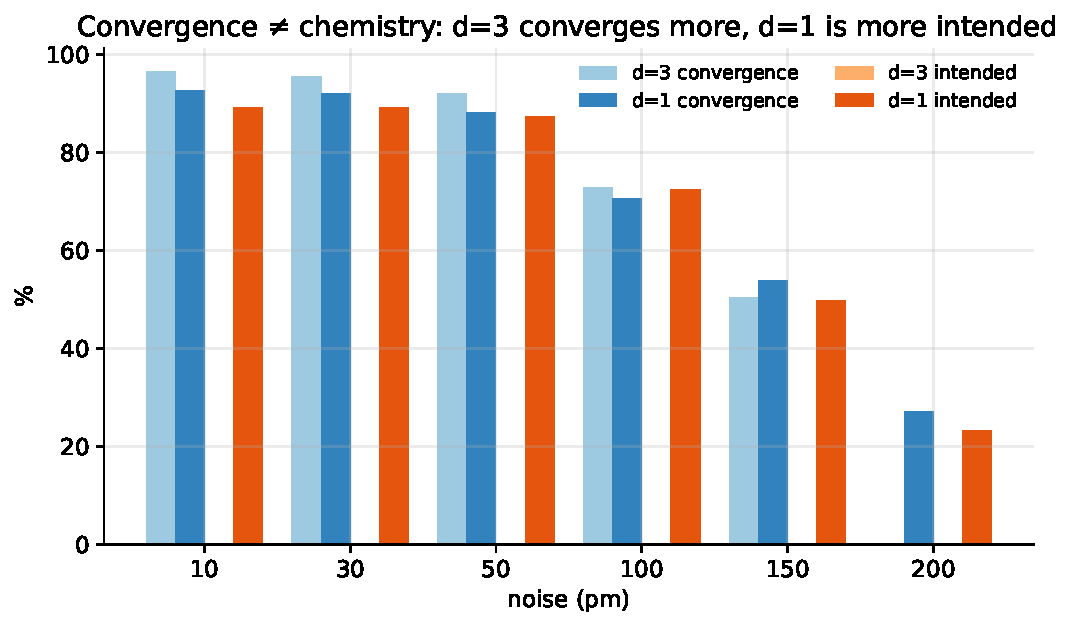
\includegraphics[width=0.8\textwidth,height=0.42\textheight,keepaspectratio]{figures_new/fig_d1_vs_d3.pdf}
\caption{\textbf{Convergence $\neq$ chemistry.} Sella d=3 converges more often than d=1 at low noise yet recovers the intended reaction \emph{less} often at every noise level --- a stale Hessian buys convergences that are not the intended TS.}
\label{fig:gal6}
\end{figure}
\begin{figure}[htbp]\centering
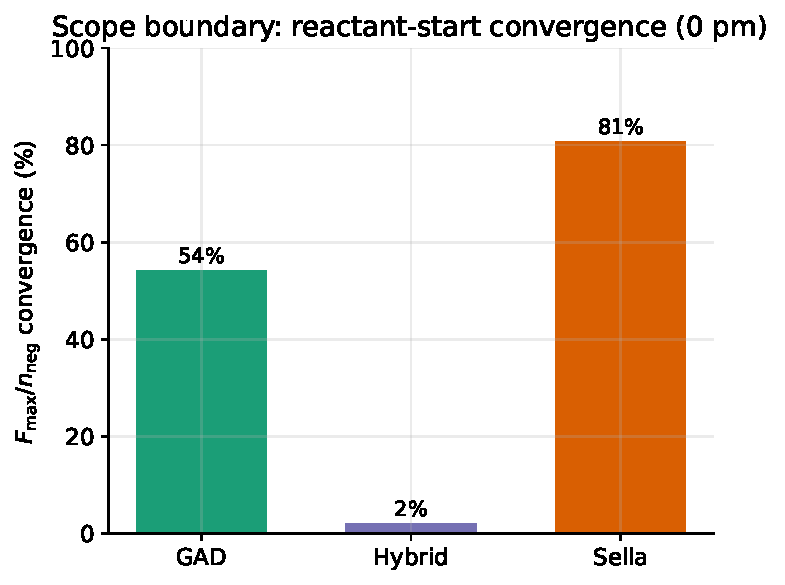
\includegraphics[width=0.55\textwidth,height=0.42\textheight,keepaspectratio]{figures_new/fig_reactant_scope.pdf}
\caption{\textbf{Scope boundary.} From a reactant start the GAD family is weak and Sella wins; GAD needs a near-saddle guess for the reaction mode to be identifiable.}
\label{fig:gal7}
\end{figure}
\clearpage

\end{document}
